\documentclass[leqno, openany]{memoir}
\setulmarginsandblock{3.5cm}{3.5cm}{*}
\setlrmarginsandblock{3cm}{3.5cm}{*}
\checkandfixthelayout

\usepackage{amsmath}
\usepackage{amssymb}
\usepackage{amsthm}
%\usepackage{MnSymbol}
\usepackage{bm}
\usepackage{accents}
\usepackage{mathtools}
\usepackage{tikz}
\usetikzlibrary{calc}
\usetikzlibrary{automata,positioning}
\usepackage{tikz-cd}
\usepackage{forest}
\usepackage{braket} 
\usepackage{listings}
\usepackage{mdframed}
\usepackage{verbatim}
\usepackage{physics}
\usepackage{stmaryrd}
\usepackage{mathrsfs} 
%\usepackage{/home/patrickl/homework/macaulay2}

%font
\usepackage[osf]{mathpazo}
\usepackage{microtype}

%CS packages
\usepackage{algorithmicx}
\usepackage{algpseudocode}
\usepackage{algorithm}

% typeset and bib
\usepackage[english]{babel} 
\usepackage[utf8]{inputenc} 
\usepackage[backend=biber, style=alphabetic]{biblatex}
\usepackage[bookmarks, colorlinks, breaklinks]{hyperref} 
\hypersetup{linkcolor=black,citecolor=black,filecolor=black,urlcolor=black}

% other formatting packages
\usepackage{float}
\usepackage{booktabs}
\usepackage{enumitem}
\usepackage{csquotes}
\usepackage{titlesec}
\usepackage{titling}
\usepackage{fancyhdr}
\usepackage{lastpage}
\usepackage{parskip}

\usepackage{lipsum}

% delimiters
\DeclarePairedDelimiter{\gen}{\langle}{\rangle}
\DeclarePairedDelimiter{\floor}{\lfloor}{\rfloor}
\DeclarePairedDelimiter{\ceil}{\lceil}{\rceil}


\newtheorem{thm}{Theorem}[section]
\newtheorem{cor}[thm]{Corollary}
\newtheorem{prop}[thm]{Proposition}
\newtheorem{lem}[thm]{Lemma}
\newtheorem{conj}[thm]{Conjecture}
\newtheorem{quest}[thm]{Question}

\theoremstyle{definition}
\newtheorem{defn}[thm]{Definition}
\newtheorem{defns}[thm]{Definitions}
\newtheorem{con}[thm]{Construction}
\newtheorem{exm}[thm]{Example}
\newtheorem{exms}[thm]{Examples}
\newtheorem{notn}[thm]{Notation}
\newtheorem{notns}[thm]{Notations}
\newtheorem{addm}[thm]{Addendum}
\newtheorem{exer}[thm]{Exercise}

\theoremstyle{remark}
\newtheorem{rmk}[thm]{Remark}
\newtheorem{rmks}[thm]{Remarks}
\newtheorem{warn}[thm]{Warning}
\newtheorem{sch}[thm]{Scholium}


% unnumbered theorems
\theoremstyle{plain}
\newtheorem*{thm*}{Theorem}
\newtheorem*{prop*}{Proposition}
\newtheorem*{lem*}{Lemma}
\newtheorem*{cor*}{Corollary}
\newtheorem*{conj*}{Conjecture}

% unnumbered definitions
\theoremstyle{definition}
\newtheorem*{defn*}{Definition}
\newtheorem*{exer*}{Exercise}
\newtheorem*{defns*}{Definitions}
\newtheorem*{con*}{Construction}
\newtheorem*{exm*}{Example}
\newtheorem*{exms*}{Examples}
\newtheorem*{notn*}{Notation}
\newtheorem*{notns*}{Notations}
\newtheorem*{addm*}{Addendum}


\theoremstyle{remark}
\newtheorem*{rmk*}{Remark}

% shortcuts
\newcommand{\Ima}{\mathrm{Im}}
\newcommand{\A}{\mathbb{A}}
\newcommand{\G}{\mathbb{G}}
\newcommand{\N}{\mathbb{N}}
\newcommand{\R}{\mathbb{R}}
\newcommand{\C}{\mathbb{C}}
\newcommand{\Z}{\mathbb{Z}}
\newcommand{\Q}{\mathbb{Q}}
\renewcommand{\k}{\Bbbk}
\renewcommand{\P}{\mathbb{P}}
\newcommand{\M}{\overline{M}}
\newcommand{\g}{\mathfrak{g}}
\newcommand{\h}{\mathfrak{h}}
\newcommand{\n}{\mathfrak{n}}
\renewcommand{\b}{\mathfrak{b}}
\newcommand{\ep}{\varepsilon}
\newcommand*{\dt}[1]{%
   \accentset{\mbox{\Huge\bfseries .}}{#1}}
\renewcommand{\abstractname}{Official Description}
\newcommand{\mc}[1]{\mathcal{#1}}
\newcommand{\msc}[1]{\mathscr{#1}}
\newcommand{\T}{\mathbb{T}}
\newcommand{\mf}[1]{\mathfrak{#1}}
\newcommand{\mr}[1]{\mathrm{#1}}
\newcommand{\ms}[1]{\mathsf{#1}}
\newcommand{\ol}[1]{\overline{#1}}
\newcommand{\ul}[1]{\underline{#1}}
\newcommand{\wt}[1]{\widetilde{#1}}
\newcommand{\wh}[1]{\widehat{#1}}
\renewcommand{\div}{\operatorname{div}}
\newcommand{\bir}{\sim_{\mr{bir}}}

\DeclareMathOperator{\Der}{Der}
\DeclareMathOperator{\Bl}{Bl}
\DeclareMathOperator{\NE}{NE}
\DeclareMathOperator{\Hom}{Hom}
\DeclareMathOperator{\End}{End}
\DeclareMathOperator{\ad}{ad}
\DeclareMathOperator{\Aut}{Aut}
\DeclareMathOperator{\Rad}{Rad}
\DeclareMathOperator{\Pic}{Pic}
\DeclareMathOperator{\supp}{supp}
\DeclareMathOperator{\sgn}{sgn}
\DeclareMathOperator{\spec}{Spec}
\DeclareMathOperator{\Spec}{Spec}
\DeclareMathOperator{\proj}{Proj}
\DeclareMathOperator{\Proj}{Proj}
\DeclareMathOperator{\ord}{ord}
\DeclareMathOperator{\Div}{Div}

% Section formatting
\titleformat{\section}
    {\Large\sffamily\scshape\bfseries}{\thesection}{1em}{}
\titleformat{\subsection}[runin]
    {\large\sffamily\bfseries}{\thesubsection}{1em}{}
\titleformat{\subsubsection}[runin]{\normalfont\itshape}{\thesubsubsection}{1em}{}

\title{COURSE TITLE}
\author{Lectures by INSTRUCTOR, Notes by NOTETAKER}
\date{SEMESTER}

\newcommand*{\titleSW}
    {\begingroup% Story of Writing
    \raggedleft
    \vspace*{\baselineskip}
    {\Huge\itshape Minimal Model Program Learning Seminar \\ Spring 2021}\\[\baselineskip]
    {\large\itshape Notes by Patrick Lei}\\[0.2\textheight]
    {\Large Lectures by Joaqu\'{\i}n Moraga}\par
    \vfill
    {\Large \sffamily Zoom University}
    \vspace*{\baselineskip}
\endgroup}
\pagestyle{simple}

\chapterstyle{ell}


%\renewcommand{\cftchapterpagefont}{}
\renewcommand\cftchapterfont{\sffamily}
\renewcommand\cftsectionfont{\scshape}
\renewcommand*{\cftchapterleader}{}
\renewcommand*{\cftsectionleader}{}
\renewcommand*{\cftsubsectionleader}{}
\renewcommand*{\cftchapterformatpnum}[1]{~\textbullet~#1}
\renewcommand*{\cftsectionformatpnum}[1]{~\textbullet~#1}
\renewcommand*{\cftsubsectionformatpnum}[1]{~\textbullet~#1}
\renewcommand{\cftchapterafterpnum}{\cftparfillskip}
\renewcommand{\cftsectionafterpnum}{\cftparfillskip}
\renewcommand{\cftsubsectionafterpnum}{\cftparfillskip}
\setrmarg{3.55em plus 1fil}
\setsecnumdepth{subsection}
\maxsecnumdepth{subsection}
\settocdepth{subsection}

\begin{document}
    
\begin{titlingpage}
\titleSW
\end{titlingpage}

\thispagestyle{empty}
\section*{Disclaimer}%
\label{sec:disclaimer}

These notes were taken during the seminar using the \texttt{vimtex} package of the editor \texttt{neovim}. 
Any errors are mine and not the speakers'. 
In addition, my notes are picture-free (but will include commutative diagrams) and are a mix of my mathematical style and that of the lecturers.
If you find any errors, please contact me at \texttt{plei@math.columbia.edu}.

\vspace*{1cm}

\noindent\textbf{Seminar Website:}  \url{https://web.math.princeton.edu/~jmoraga/Learning-Seminar-MMP}
\newpage


\tableofcontents

\chapter{Overview}%
\label{cha:overview}

The goal of the minimal model program is to classify smooth projective complex varieties $X \subseteq \P^n$. Let $T_X$ be the tangent byndle and $\Omega_X$ be the cotangent bundle. Then $\omega_X = \Omega_X^n$ is called the \textit{canonical bundle}, and can be written as $\msc{O}_X(K_X)$ for some Cartier divisor $K_X$.

\begin{quest}
    Can we understand the geometry of $X$ using numerical properties of $K_X$?
\end{quest}

For a curve $C \subseteq X$ and a line bundle $\msc{L}$ on $X$, then $\msc{L}.C = \deg_C(i^* \msc{L})$. Then $K_X$ is \textit{ample (resp. antiample)} if $K_X . C > 0$ (resp $<0$) for all curves $C \subseteq X$. Similarly, $K_X$ is \textit{numerically trivial} if $K_X . C = 0$ for all curves $C \subseteq X$.

\begin{defn}
    We say that $X$ is \textit{Fano} if $K_X$ is antiample, \textit{Calabi-Yau} if $K_X$ is numerically trivial, and \textit{canonically polarized} if $K_X$ is ample.
\end{defn}

\begin{exm}
    If $C$ is a Fano curve, then $C \simeq \P^1$. If $C$ is a CY curve, then $C$ is an elliptic curve. If $C$ is a canonically polarized curve, then $g(C) \geq 2$.
\end{exm}

\begin{exm}
    Let $X \subseteq \P^n$ be a smooth hypersurface of degree $d$. Then by the adjunction formula, we have $K_X \simeq \eval{(K_{\P^n} + X)}_X \simeq \eval{(d-n-1)H}$. Therefore, $X$ is Fano if $d \leq N$, CY if $d = n+1$, and canonically polarized if $d \geq n+2$.
\end{exm}

\begin{rmk}
    If $E$ is an elliptic curve, then $E \times \P^1$ has $K_X . C = 0$ for some curves and $K_X . C < 0$ for others.
\end{rmk}

Now we consider various properties of different varieties:
\begin{table}[H]
    \centering
    \caption{Properties of varieties of different classes}
    \label{tab:label}
    \begin{tabular}{rlcl}
    \toprule
    & Fano & CY & Canonically polarized \\
    \midrule
        $\pi_1$ & trivial & {?} & generally infinite \\
        Automorphisms & linear algebraic groups & {?} & finite groups \\
        Birational automorphisms & monstrous & {?} & finite groups \\
        Geometry & simple geometry & {?} & complicated, rich \\
        Arithmetic & a lot of $\Q$-points & {?} & $\Q$-points in a proper closed \\
        \bottomrule
    \end{tabular}
\end{table}
We have said nothing about Calabi-Yaus, but of course by the Beauville-Bogomolov decomposition, we can reduce to pure Calabi-Yaus ($h^{i,0} = 0$ for $0 < i < \dim X$), hyperk\"ahlers, and abelian varieties up to taking a finite cover.

Now let $x$ be a closed point on $X$. Then there is a variety $\Bl_x X \to X$ that is an isomorphism away from $x$ where the fiber above $x$ is an exceptional divisor $E$ parameterizing tangent directions at $x$.

\begin{exm}
    Consider points $p_1, \ldots, p_n, \ldots \in \P^2$. Then if we blow up these points in a sequence, we obtain a sequence of varieties $X_1, \ldots, X_2, \ldots, X_n, \ldots$ Over $\P^2 \setminus \qty{p_1, \ldots, p_{i-1}}$, the morphism $X_i \to \P^2$ is an isomorphism. For $i \neq j$, clearly $X_i$ is not isomorphic to $X_j$ (they have different Picard ranks), but they are \textit{birational}. We say that $X_1 \bir X_2$ if they have isomorphic dense open subsets.
\end{exm}

Now we can state the goal of the Minimal Model Program. If $X$ is projective and has ``mild singularities'' the goal is to prove that there exists a birational map $\pi \colon X \dashrightarrow X'$ and a fibration ($\varphi_* \msc{O}_{X'} = \msc{O}_Z$ and positive dimensional general fiber) $X' \xrightarrow{\varphi} Z$ such that one of the following holds:
\begin{enumerate}
    \item $F$ is Fano;
    \item $F$ is Calabi-Yau;
    \item $Z = \Spec \C$ and $X'$ is canonically polarized.
\end{enumerate}
The way we will construct this birational morphism is by studying the geometry of curves on $X$ which intersect $K_X$ negatively. If $K_X.C < 0$ under some hypotheses (extremity on $NE(X)$), we can find $\varphi_C \colon X \to X_1$ contracting precisely the curves which are numerically equivalent to a positive multiple of $C$.

\begin{enumerate}
    \item If the curves numerically equivalent to a positive multiple of $C$ cover $X$, then $\varphi_C$ has positive-dimensional fibers, is a contraction, and the general fiber $F$ is Fano. This is called a \textit{Mori fiber space}.
    \item If the curves numerically equivalent to a positive multiple of $C$ cover a divisor on $X$, then we say that $\varphi_C \colon X \to X_1$ is a divisorial contraction and thus $\rho(X_1) = \rho(X) - 1$. $X_1$ still has nice singularities, so we can iterate this process.
    \item The last case is called a small contraction. The curves which are numerically equivalent to a positive multiple of $C$ cover a set of codimension at least $2$. In this case, $X_1$ may have very bad singularities (by this, we mean that $K_{X_1}$ is not $\Q$-Cartier). We construct a new birational morphism $\varphi_C^+ \colon X^+ \to X_1$ which contracts $K_{X^+}$-positive curves.
\end{enumerate}

Another type of surgery is a flip, which changes a locus of codimension at least $2$. For example, consider $D = p_1^* \msc{O}(1) \otimes p_2^* \msc{O}(r)$ on $\P^1 \times \P^1$. Then write
\[ X = \Spec \qty(\bigoplus_{m \geq 0} H^0 (\P^1 \times \P^1, \msc{O}_{\P^1 \times \P^1}(mD))). \]
Then $X$ is (locally) a cone over $\P^1 \times \P^1$, so $K_X$ is not $\Q$-Cartier. Therefore, we can blow up the vertex, and the exceptional divisor is $E \simeq \P^1 \times \P^1$. Now the $\P^1 \times \P^1$ can be collapsed onto each of the two factors, so we obtain a birational map $\pi \colon X_1 \dashrightarrow X_1^+$. Here, if $C,C^+$ are the resulting curves, we have $K_{X_1}.C < 0$ and $K_{X_1^+}.C^+ > 0$.
\begin{figure}[H]
    \centering
    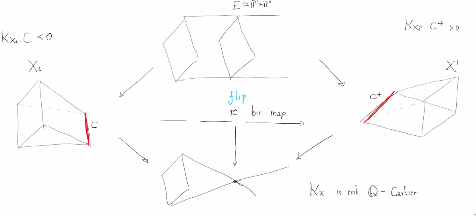
\includegraphics[width=0.8\linewidth]{flip}
    \caption{A Flip}%
    \label{fig:flip}
\end{figure}
This gives us the question:
\begin{quest}
    Do flips always exist?
\end{quest}
Now either the algorithm given by iterating this process always terminates or it continues infinitely. We are fine once we reach the Mori fiber space case, and there are only $\rho(X) - 1$ divisorial contractions, so the only possible problem is that there is an infinite sequence of flips.

\begin{conj}[Termination of flips]
    This algorithm always terminates after finitely many flips with either a Mori fiber space $X_n \to Z$ or a variety $X_n$ such that $K_{X_n}.C \geq 0$ for every curve $C$ (in other words, $K_{X_n}$ is nef).
\end{conj}

\begin{conj}[Abundance]
    $X$ has mild singularities and $K_X$ is nef. Then $\abs{m K_X}$ is basepoint-free for some $m \gg 0$.
\end{conj}

If this is true, and $X \xrightarrow{\varphi} X_1$ contracts all $K_X$-trivial curves, then either
\begin{enumerate}
    \item The general fiber has positive dimension. In this case, $K_F \equiv 0$.
    \item $\dim X = \dim X_1$. Then $X \to X_1$ is birational and $X_1$ is canonically polarized.
\end{enumerate}

Therefore, the goal of the MMP is achieved if we can solve the conjectures of existence of flips, termination of flips, and abundance. Existence of flips was proved by Birkar, Cascini, Hacon, and McKernan in 2006 and termination is known in dimension at most $3$ and in some cases in dimension $4$. Finally, abundance is known in dimension at most $3$.

\chapter{MMP in Dimension $3$}%
\label{cha:mmp_in_dimension_3_}

\section{Rational Curves}%
\label{sec:bend_and_break}

\begin{prop}[Bend and Break]
    Let $X$ be proper and $C$ be a smooth proper curve. Let $p \in C$ and $g_0 \colon C \to X$ be nonconstant. Next, let $0 \in D$ be a pointed curve and $G \colon C \times D \to X$ such that
    \begin{enumerate}
        \item $\eval{G}_{C \times \qty{0}} = g_0$.
        \item $G(\qty{p} \times D) = g_0(p)$.
        \item $\eval{G}_{C \times \qty{t}}$ is different from $g_0$ for general $t$.
    \end{enumerate}
    All of these imply that this is a nontrivial deformation of $g_0$ fixing $p$. Then there exists $g_1 \colon C \to X$ and $Z = \sum a_i Z_i$ a union of rational curves such that ${(g_0)}_* C$ is algebraically equivalent to ${(g_1)}_* (C) + Z$ and $g_0(p) \in \bigcup_i Z_i$. In particular, there exists a rational curve through $g_0(p)$.
\end{prop}

\begin{proof}
    First, compactify $D$ and let $\ol{G} \colon C \times \ol{D} \dashrightarrow X$ be the rational map. This map is undefined at $\qty{p} \times \ol{D}$ by the rigidity lemma, so let $S$ be the normalization of the graph of $\ol{G}$. So we have a map $\pi \colon S \to C \times \ol{D}$ and write $G_S \colon S \to $. 

    Then we define $h \colon S \to C \times \ol{D} \to \ol{D}$. Then there exist $d \in C \times \ol{D}$ such that $\pi$ is not an isomorphism over $d$. Then we know that $h^{-1}(d) = C' + E$ where $C'$ is a birational transform of $C$ and $E$ is $\pi$-exceptional. Then we set $g_1 \colon C \to X$ to be the restriction of $G_S$ to $C'$ and $Z = G_S(E)$.

    By a lemma of Abhyankar, we know that $E$ is a union of rational curves, and then by the L\"uroth theorem, we know that $Z$ is a union of rational curves and
    \[ {(g_0)}_* C \sim_{\mr{alg}} {(g_1)}_* C + Z. \]
\end{proof}

\begin{lem}[Abhyankar]
    Let $X$ have mild singularities and $Y \xrightarrow{\pi} X$ be a proper birational morphism. For any $x \in X$, either $\pi^{-1}(x)$ is a point or is covered by rational curves.
\end{lem}

Here is an intuitive image of the bend-and-break process:
\begin{figure}[H]
    \centering
    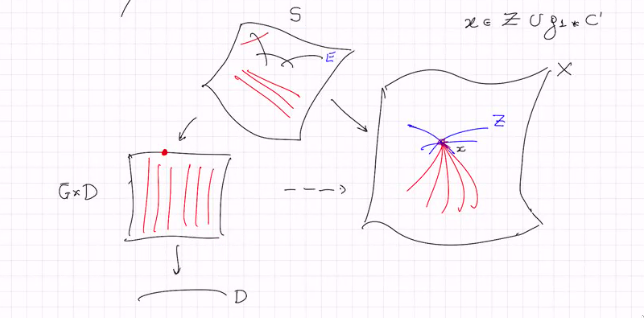
\includegraphics[width=0.8\linewidth]{bendbreak}
    \caption{Bend and Break}%
    \label{fig:bendbreak}
\end{figure}

\begin{prop}[Bend and Break II]
    Let $X$ be a projective variety and $g_0 \colon \P^1 \to X$ be a nonconstant morphism. Let $D$ be a smooth pointed curve and $G \colon \P^1 \times D \to X$ such that
    \begin{enumerate}
        \item $\eval{G}_{\P^1 \times \qty{0_D}} = g_0$;
        \item $G(\qty{0} \times D) = g_0(0), G(\qty{\infty} \times D) = g_0(\infty)$;
        \item $G(\P^1 \times D)$ is a surface.
    \end{enumerate}
    Then ${(g_0)}_* \P^1$ is algebraically equivalent either to a reducible curve or a multiple curve.
\end{prop}

\begin{proof}
    Let $S$ be a $\P^1$-bundle containing $\P^1 \times D$ and consider the rational map $\wt{G} \colon S \dashrightarrow X$. Then we can resolve the basepoints to obtain $\wt{G} \colon \wt{S} \to S$ and induct on $\rho(\wt{S} / S) \eqqcolon \rho$.
    \begin{description}
        \item[Case 1: $\rho = 0$:] Consider the sections $C_0, C_{\infty}$ at $0$ and $\infty$. Then let $H$ is ample on $X$ and then we see that ${(\wt{G}^* H)}^2 > 0$ and ${(C_0 \cdot \wt{G}^* H)} = {(C_{\infty} \cdot \wt{G}^* H)} = 0$ by the projection formula. By the Hodge index theorem, we see that $C_0^2 < 0, C_{\infty}^2 < 0$ (because $\wt{G}^* H, C_0, C_{\infty}$ are linearly independent). But then we know that $\rho(S) = 2$, which is a contradiction.
        \item[Inductive step:] Consider the diagram
            \begin{equation*}
            \begin{tikzcd}
                \wt{S} \ar{rr}{\wt{G}} \ar{d}{r'} \ar[swap,bend right=40]{dd}{\wt{r}} & & X \\
                S' \ar{d}{r} \ar[dashrightarrow]{urr}{\ol{G}'} \\
                S \ar{d}{q} \ar[swap,dashrightarrow]{uurr}{\ol{G}} \\
                D.
            \end{tikzcd}
            \end{equation*}
            Then $r$ is the first blowup in $\wt{S} \to S \ni P$ and $y \in D$ will be a point such that $P \in q^{-1}(y)$. Let $F_1$ be the exceptional divisor of $r$ and $F_2$ be the strict transform of $q^{-1}(y)$ in $S'$. Then $F_1, F_2$ intersect at a point $Q$. But then $\ol{G}'$ is a morphism around $F_2$. But then ${(g_0)}_* \P^1 \sim \wt{G}_* ({(q \circ r)}^* (y))$, which is reduced and irreducible. If $\ol{G}$ is not defined at $Q \neq P$, then
            \[ \wt{G}_* ({(q \circ r)}^* (y)) = \wt{G}_* \mr{red}(\wt{r}^{-1}(p)) + \wt{G}_* \mr{red} (\wt{r}^{-1}(Q)) + (\text{effective}), \]
            which is a contradiction and thus $\ol{G}$ is defined at $Q \neq P$. Then if $\ol{G}'$ is not defined at $Q_0$, then after blowing up $Q_0$, we see that ${(q \circ r)}^* (y)$ must contain a component of multiplicity at least $2$. Now contracting $F_2$, we have the desired result by induction on $\rho$. \qedhere
    \end{description}
\end{proof}

This tells us that to produce rational curves, we simply need to deform them with enough fixed points and use bend and break. But now we need to actually find rational curves.

\begin{thm}
    Let $X$ be smooth and projective and $-K_X$ be ample. For every $x \in X$, there exists a rational curve $C$ through $x$ such that
    \[ 0 < -K_X . C \leq \dim X + 1. \]
\end{thm}

\begin{proof}
    Choose some curve $C \subseteq X$ through $x$. Then the space of deformations of $C$ on $X$ fixing $x$ has dimension at least
    \[ h^0(C, f^* T_X) - h^1(C, f^* T_X) - \dim X = - f_* C. K_X - g(C) \dim X. \]
    We have several cases:
    \begin{enumerate}
        \item If $g(C) = 0$, then we are done.
        \item If $g(C) = 1$, then we can replace $f$ with the composition by an endomorphism of large degree $n$, then we see that
            \[ - ({(f \circ h)}_* C \cdot K_X) - \dim X = -n^2 f_* C.K_X - \dim X > 0 \]
            whenever $n$ is sufficiently large
        \item Assume $g(C) \geq 2$. Then there are no endomorphisms of high degree, so assume $X, C$ are defined over $\Z$. Then let $X_p, C_p$ be the reduction to $\ol{F}_p$. Now we apply the Frobenius map $F_p$, which has degree $p$. By generic flatness, we know that ${(f_p)}_* C_p.K_{X_p}, g(C_p), \chi\qty(\eval{T_X}_{C_p})$ are the same for almost all $p$, so by the same argument as in the genus $1$ case, we see have a rational curve $A_p$ on $X_p$ for almost all $p$. By bend and break II, we can find a rational curve of the desired degree.

            Then we use the fact that if a statement holds for all $p$ large enough, then it holds for the complex numbers, and we obtain a curve. This is analogous to the idea that if $Z \subseteq \P^n_{\Z}$, then if the image of $\pi \colon Z \to \Spec \Z$ contains a Zariski-dense subset, then it contains the generic point. \qedhere
    \end{enumerate}
\end{proof}

\begin{thm}
    Let $X$ be a smooth projective variety and let $H$ be ample on $X$. Assume there exists $C' \subseteq X$ such that $-(C'.K_X) > 0$. Then there exists a rational curve $E$ such that $\dim X + 1 \geq -(E.K_X) > 0$ and
    \[ \frac{-(E.K_X)}{E.H} \geq \frac{-C'.K_X}{C'.H}. \]
\end{thm}

\begin{thm}[Cone Theorem]
    Let $X$ be smooth and projective. Then there exist countably many curves $C_r \subseteq X$ such that $0 < - K_X.C_i \leq \dim X + 1$ and 
    \[ \ol{\NE}(X) - {\ol{\NE}(X)}_{K_X \geq 0} + \sum_i \R_{\geq 0} [C_i]. \]
\end{thm}

\begin{proof}
    Choose $C_i$ with $0 < -(C.K_X) \leq \dim X + 1$ and let $W$ be the closure of $\ol{\NE}_{K \geq 0} + \sum_i \R_{\geq 0} [C_i]$. Now choose $D$ positive on $W \setminus \qty{0}$ and negative somewhere on $\ol{\NE}(X)$. Let $H$ be ample and 
    \[ \mu = \max \qty{\mu' \mid H + \mu' D\ \text{is nef}}. \] 
    This means that $H + \mu D$ is nef. Then let $Z \in \ol{\NE}(X)$ with $(H+\mu D).Z = 0$ and $K_X.D < 0$. Let $Z_k$ be a sequence of curves approximating $Z$. Then we see that
    \[ \max_j \frac{- (Z_{k_j}. K_X)}{(Z_{k_j}.(H + \mu'D))} \geq \frac{-Z_k.K_X}{Z_k.(H+\mu D)} \]
    is obtained by $Z_{k_0}$. Now we will replace $Z_k$ with rational curves $E_{i(k)}$ such that $\dim X + 1 \geq - E_{i(k)}.K_X > 0$ and 
    \[ \frac{-E_{i(k)}.K_X}{E_{i(k)}.(H + \mu' D)} \geq \frac{-Z_{k_0}.K_X}{Z_{k_0}.(H+\mu'D)} \geq \frac{-Z_k.K_X}{Z_k.(H+\mu'D)}. \]
    Because $E_{i(k)}.D \geq 0$, we have
    \[ \frac{-E_{i(k)}.K_X}{E_{i(k)}.H} \geq \frac{-Z_k.K_X}{Z_k.(H+\mu'D)}. \]
    Fixing $M \gg 0$ such that $MH + K_X$ is ample, then we see that $(MH + K_X).E_{i(k)} > 0$, so
    \[ M > \frac{- E_{i(k)}.K_X}{E_{i(k)}.H} \geq \frac{-Z_k.K_X}{Z_k.(H+\mu'D)}. \]
    Taking $k \to \infty, \mu' \to \mu$, we see that
    \[ M > \frac{Z.K_X}{Z.(H+\mu D)} \longrightarrow \infty, \]
    a contradiction.
\end{proof}

\begin{exm}
    Suppose $K_X$ is not nef. Then there are no rational curves on $X$. For example, there are no rational curves of an abelian variety.
\end{exm}

\section{Singularities of the MMP}%
\label{sec:singularities_of_the_mmp}

Consider pairs $(X, \Delta)$ such that $X$ is normal quasiprojective and $K_X + \Delta$ is $\Q$-Cartier. These are called \textit{log pairs}. 

\begin{defn}
    Let $\pi \colon Y \to X$ is a resolution of singularities, $E \subseteq Y$ is exceptional, and $\pi^* (K_X + D) + \sum E_i$ has simple normal crossings. Define the \textit{log discrepancy} 
    \[ a_E(X, D) \coloneqq 1 + \operatorname{coeff}_E (K_Y - \pi^* (K_X + D)). \]
\end{defn}

\begin{defn}
    We say that $(X, \Delta)$ is 
    \begin{enumerate}
        \item \textit{terminal} if $a_E(X, \Delta) > 1$ for every exceptional $E$ over $Y$.
        \item \textit{canonical} if $a_E(X, \Delta) \geq 1$ for every exceptional $E$ over $Y$.
        \item \textit{Kawamata log terminal} if $a_E(X, \Delta) > 0$ for every $E$.
        \item \textit{log canonical} if $a_E(X, \Delta) \geq 0$ for every $E$.
    \end{enumerate}
\end{defn}

Now if $X$ is smooth projective and $K_X$ is pseudoeffective, then there exists $X \dashrightarrow X_{\mr{ter}}$ such that $K_{X_{\mr{ter}}}$ is nef. By abundance, $K_{X_{\mr{ter}}}$ is semiample. Then there is a morphism $X_{\mr{ter}} \to X_{\mf{can}}$ such that $K_{X_{\mr{can}}}$ is ample. Then terminal singularities are those that may appear in the terminal model, and canonical singularities are those that may appear on the canonical model.

Recall the \textit{adjunction formula}: If $(X, D)$ is log smooth, then $K_X + \eval{D}_D \sim K_X$. Usually, $(X,D)$ is log canonical but not klt. But then $a_D(X,D) = 0$ but $a_E(X, D) > 0$ for every $E \neq D$. Terminal singularities are the smallest category of singularities that we need to understand to run the minimal model program. On the other hand, log canonical is the largest class of singularities in which we can expect the MMP to work.

\begin{exm}[Examples of klt singularities]
    Both cone singularities and quotient singularities are klt. 
\end{exm}

\begin{prop}[Cones]
    Let $(X, \Delta)$ be a log pair and $A$ an ample Cartier divisor on $X$. Then define
    \[ C(X, \Delta) = \Spec (\bigoplus_{m \geq 0} H^0(X, \msc{O}_X(mA))). \]
    Then $C(X, A)$ is 
    \begin{enumerate}
        \item terminal if and only if $rA \sim_{\Q} K_X + \Delta$ with $r < -1$ and $(X, \Delta)$ terminal;
        \item canonical if and only if $ra \sim_{\Q} k_x + \delta$ with $r \leq -1$ and $(X, \Delta)$ canonical;
        \item klt if and only if $ra \sim_{\Q} k_x + \delta$ with $r < 0$ and $(X, \Delta)$ is klt;
        \item log canonical if and only if $ra \sim_{\Q} k_x + \delta$ with $r \leq 0$ and $(X, \Delta)$ is log canonical.
    \end{enumerate}
    In particular, the cone over a Fano is klt, the cone over a Calaby-Yau is log canonical, and cones over canonically polarized varieties are terrible.
\end{prop}

\begin{exm}
    Consider the cone $C_n$ over a rational normal curve of degree $n$. Then resolving $Y_n \to C_n$, we see that the exceptional $E_n \simeq \P^1$ and 
    \[ \pi^* (K_{C_n}) = K_{Y_n} + \qty(1 - \frac{2}{n}) E_n, \] 
    and therefore $a_{E_n}(C_n) = \frac{2}{n}$.

    Consider $E \subseteq \P^3$ and elliptic curve. Then $\pi^*(K_{C_E}) = K_{Y_E} + E$, so $a_E(C_E) = 0$.
\end{exm}

Now consider $G \subseteq GL_n$ a finite group. Then $\C^n/G = \Spec {\C[x_1, \ldots, x_n]}^G$ has klt singularities.

\begin{exm}
    In dimension $2$, we have
    \begin{enumerate}
        \item terminal is equivalent to smooth;
        \item canonical is equivalent to ADE;\@
        \item klt is equivalent to quotient singularity;
        \item log canonical is ``equivalent'' to quotient and/or elliptic cone.
    \end{enumerate}
\end{exm}

\begin{exm}
    In dimension $3$, terminal singularities are classified as quotients of hypersurface singularities, also known as \textit{hyperquotient singularities}. Then are given by actions of finite groups $G$ acting on hypersurface singularities of the form $\qty{x^2 + y^2 + f(z, w) = 0}$. Even for canonical singularities, we have no idea what they look like.
\end{exm}

\begin{exm}
    In dimension $4$, there are examples of $4$-fold terminal singularities with analytic embedding dimension $n$ for every $n$ (Kollar, 2010). By contrast, terminal singularities in dimension $3$ all have analytic embedding dimension $4$.
\end{exm}

\begin{thm}[Prokhorov, Xu, 2019]
    Any klt singularity deforms to a klt cone singularity. For $x \in X$, there exists a flat morphism $\msc{X} \xrightarrow{\varphi} \A^1$ such that $\varphi(\A^1 \setminus 0) \sim (\A^1 \setminus 0) \times X$ and $\varphi^{-1}(0) = X_0$ is a klt cone singularity. This is just a deformation to the normal cone.
\end{thm}

We will apply the following philosophy: 
\begin{quotation}
    \textit{Any theorem for smooth projective varieties should work with klt singularities}. 
\end{quotation}

\begin{exm}
    Let $K_X = 0$. By Beauville-Bogomolov (1970s), there exists a cover $X \gets Y$, where $Y$ is a product of abelian varieties, irreducible Calabi-Yau varieties, and hyperk\"ahlers. There is an analogue for klt singularities that was proved by Druel, Campana,\ldots in 2020.
\end{exm}

\begin{exm}
    Let $X$ be smooth projective and $-K_X$ be nef. Then 
    \[ \wt{X} \sim \C^q \times \prod Y_i \times \prod S_k \times Z, \]
    where $Y_i$ is strict Calabi-Yau, $S_k$ is hyperkahler, and $Z$ is rationally connected. There is a version for klt singularities in progress.
\end{exm}

We will now discuss localization of singularities. Suppose $X$ is a variety with terminal singularities and $Z \subseteq X$ a subvariety of codimension $1$. Then $\Spec \msc{O}_{X,Z}$ has terminal singularities if and only if $\Spec \msc{O}_{X,Z}$ is a smooth local ring, and this is equivalent to smoothness at the generic point of $Z$. In particular, if $X$ is terminal, the singularities must appear in codimension at least $3$.

\section{Vanishing}%
\label{sec:vanishing}

Let $C \subseteq X$ be a $K_X$-negative curve. Then if $K_X \sim_{\Q} E \geq 0$ for some $E$ effective, we see that $K_X.C = E.C < -$, so $C \subseteq E$. Now if $(X, D)$ is a log smooth pair, we have an exact sequence
\[ 0 \to \msc{O}_X(K_X) \xrightarrow{\otimes D} \msc{O}_X (K_X \times D) \to \msc{O}_D(K_D) \to 0. \]
If $H^1(X, \msc{O}_X(K_X)) = 0$, then $H^0(K_X + D) \twoheadrightarrow H^0(K_D)$. This tells us that vanishing theorems help us find sections of line bundles.

\begin{thm}[Kodaira Vanishing]
    Let $X$ be smooth projective and $\msc{L}$ be ample. Then $H^i(X, \msc{L}^{-1}) = 0$ for all $i < \dim X$.
\end{thm}

\begin{proof}[Sketch of Proof]
    Let $s \in H^0(X, \msc{L}^m)$ and $D = (s=0)$ be smooth. Then we have $\msc{O}_X \xrightarrow{s} \msc{L}^m$. Now we have
    \[ \msc{L}^{-i} \otimes \msc{L}^{-j} \simeq \msc{L}^{-i-k} \msc{O}_X \xrightarrow{\mr{id} \otimes s} \msc{L}^{-i-j} \otimes \msc{L}^m = \msc{L}^{-i-j+m}. \]
    Setting $Z = \Spec \bigoplus_{i=0}^{m-1} \msc{L}^{-i}$ with projection $p \colon Z \to X$, we note that if $X, D$ are smooth, then $Z$ is smooth. Consider a morphism $\tau \colon H^i(Z, \C_Z) \twoheadrightarrow H^i(Z, \msc{O}_Z)$ and its pushforward $p_* \tau \colon H^i(X, p^* \msc{C}_Z) \twoheadrightarrow H^i(X, p_* \msc{O}_Z)$. Now we consider the surjection
    \[ \bigoplus_{r=0}^{m-1} H^i(X, \C[\zeta^r]) \twoheadrightarrow \sum_{r=0}^{m-1} H^i\qty(X, \bigoplus_{r=0}^{m-1} \msc{L}^{-r}). \]
    Now we use the result that $\C[\zeta^r] \hookrightarrow \msc{L}^{-r}$ factors through $\C[\zeta^r] \hookrightarrow \msc{L}^{-r}(-k D) \hookrightarrow \msc{L}^{-r}$. By Serre, we see that $H^i(X, \msc{L}^{-(r+mk)}) = 0$ for arbitrary $k$.
\end{proof}

\begin{thm}[KV vanishing]
    Let $X$ be a smooth projective complex and $\msc{L}$ be a line bundle on $X$ such that $\msc{L} \equiv M + \sum a_i D_i$, where $M$ is a big and nef $\Q$-divisor, $\sum D_i$ is a snc divisor, and $0 \leq a_i < 1, a_i \in \Z$. Then $H^i(X, \msc{L}^{-1}) = 0$ for $i < \dim X$.
\end{thm}

\begin{prop}
    Let $X$ be quasiprojective and normal, $D$ Cartier, and $m > 0$ a positive integer. Suppose $Y \xrightarrow{p} X$ is finite and $D'$ Cartier such that $p^* D \sim MD'$. If $X$ is smooth and $\sum F_j$ is simple normal crossing, then $Y$ is smooth and $\sum p^* F_j$ has simple normal crossings.
\end{prop}

\begin{lem}
    Let $Y \to X$ be finite. Then $\msc{O}_X \to f_* \msc{O}_Y$ splits. If $\msc{F}$ is a coherent sheaf on $X$, then $\msc{F}$ is a direct summand of $f_* f^* \msc{F}$. Finally, $H^i(X, \msc{F})$ is a direct summand of $H^i(Y, f^* \msc{F})$.
\end{lem}

\begin{proof}[Sketch of KV Vanishing]
    Consider $\sum a_i D_i$ and write $a_1 = b/m$ for some $m \geq 0$. Then consider $p_1 \colon X_1 \to X$ such that $p^* D_1 \sim m D$. Then $H^i(X, \msc{L}^{-1})$ is a direct summand of $H^i(X_1, p_1^* \msc{L}^{-1})$. Then $p_1^* D_1$ is a section of $\msc{O}_X(mD)$, so we can apply the index cover to obtain $X_2 \xrightarrow{p_2} X$ with $X_2$ smooth, $p_2^* (D_i)$ is smooth, and $\sum p_2^* p_1^* D_i$ has simple normal crossings. Then
    \[ {(p_2)}_* \msc{O}_{X_2} = \sum_{k=0}^{m-1} \msc{O}_{X_1}(-j D), \]
    so
    \[ H^i(X_2, p_2^* p_1^* \msc{L}^{-1}(b D)) = \bigoplus_{j=0}^{m-1} H^i(X, p_1^* ((b-j)D)). \]
    Choosing $j = b$, we see that $H^i(X_1, p_1^* \msc{L}^{-1})$ is a direct summand of $H^i(X_2, p_2^* p_1^* \msc{L}^{-1}(bD))$. Therefore, 
    \[ p_2^* p_1^* \msc{L}^{-1}(bD) = p_2^* p_1* M + \sum_{i > 1} a_1 p_2* p_1* (D_i). \]
    But now we have reduced the number of components of $D_i$, so by induction, the cohomology of the pullback vanishes. Now we need to consider $M$. We know $M$ is big and nef, so $M \sim_{\Q} A + E$, where $A$ is ample and $E$ is effective. Then there exists $f \colon Y \to X$ projective and birational such that $f^* \msc{L} = A + E$, where $A$ is ample and $E$ has simple normal crossings with $E = \sum a_i E_i, 0 \leq a_i < 1$. Now let $H \subseteq X$ be an ample divisor. Then
    \[ H^i(X, \msc{L}(rH) \otimes R^j f_* \omega_Y) \Rrightarrow H^{i+j}(Y, \omega_Y \otimes f^* \msc{L}(rH)). \]
    But then $f^* \msc{L}(rH) = (A + r f^* H) + E$, where $A + rf^* H$ is ample. But now we know that
    \[ H^k(Y, f^* \msc{L}(rH) \otimes \omega_Y) = 0 \]
    for $k > 0$, so 
    \[ H^0(X, \msc{L}(rH) \otimes R^j f_* \omega_Y) = H^j(Y, \omega_Y \otimes f^* \msc{L}(rH)) = 0 \]
    and therefore $R^j f_* \omega_Y = 0$ for $j > 0$. But now setting $r = 0$, we see that
    \[ H^i(X, \msc{L} \otimes f_* \omega_Y) \simeq H^i(Y, f^* \msc{L} \otimes \omega_Y) = 0. \qedhere \]
\end{proof}

\begin{thm}
    Let $(X, \Delta)$ be a proper klt pair with $N$ a $\Q$-Cartier divisor. Suppose that $N = M + \Delta$, where $M$ is big and nef. Then $H^i(X, \msc{O}_X(-N)) = 0$ for $i < \dim X$. Equivalently, $H^{n-i}(X, K_X + N) = 0$ for $n-i > 0$.
\end{thm}

\begin{rmk}
    This philosophy fails for log canonical singularities.
\end{rmk}





\end{document}
